\begin{doublespace}

During the course of this project, three user studies were carried out in order to receive feedback about the system. The first study was conducted using the gearbox design software made by Holman and Okafor (2018), referred to as the ``old system''. This study will be referred to here as the A20 study since it was done during A term of 2020. The system that was developed for this project, named ``GearTrain'', had a study done during C term and D term 2021, and are referred to as the C21 and D21 study, respectively. Since each study has different target audiences and each software has different features, the studies will be divided in this section. All survey questions and answers can be found in Appendix~\ref{app:survey}, while all tutorial documents can be found in Appendix~\ref{app:tutorial}. Data from each study can be compared to see differences in user feedback across systems and which system users seem to prefer.

\subsection{Study of the Old System}

The study of the old system (A20) was conducted in two Introduction to CAD (ES 1310) classes at Worcester Polytechnic Institute during A term (August-October) 2020. There were a total of forty-three participants for this study, which was largely focused on what users liked about the old system and what could be improved. Most of the students in the class were freshman (Figure~\ref{fig:grades}). Full answers to some short response questions can be found in Appendix~\ref{app:survey}, while this section will provide a summary of the data.

\begin{figure}
    \centering
    \begin{tikzpicture}
        \pie{41.3/Freshman, 37/Sophomore, 13/Junior, 8.7/Senior}
    \end{tikzpicture}
    \caption{Year breakdown of study participants (A20, total=46).}
    \label{fig:grades}
\end{figure}

\subsubsection{User Demographics for A20 Study}

Each participant was asked to complete two surveys: one before they started the task and one after they completed the task. Fifty percent of participants majored in Mechanical Engineering, as CAD is something that mechanical engineers use a lot. See Figure~\ref{fig:majors} for a full breakdown of the majors in the study. ``Other'' are any other majors besides the ones listed where only one student has that as their major. For example, one student majors in Environmental Engineering, but they are placed in ``other'' since there is only one environmental engineering major. Of all forty-three participants, a total of nine students had a minor, but each minor was unique to that student except for Spanish and IMGD (Interactive Media and Game Design) which had two. See Figure~\ref{fig:minors} for a full breakdown.

\begin{figure}
    \centering
    %\includegraphics[height=0.3\paperheight, width=1\textwidth]{Majors}
    \begin{tikzpicture}
        \pie{52.2/Mechanical Engineering, 10.9/Other, 19.6/Biomedical Engineering, 13.0/Computer Science, 4.3/Industrial Engineering}
    \end{tikzpicture}
    \caption{Study participant majors (A20, total=46).}
    \label{fig:majors}
\end{figure}

\begin{figure}
    \centering
    %\includegraphics[width=1\textwidth]{Minors}
    \begin{tikzpicture}
        \pie{11.1/Computer Science, 11.1/Sustainability Engineering, 11.1/Robotics Engineering, 22.2/IMGD, 22.2/Spanish, 11.1/Materials Engineering, 11.1/Environmental Engineering}
    \end{tikzpicture}
    \caption{Study participant minors (A20, total=9).}
    \label{fig:minors}
\end{figure}

\subsubsection{Previous Experience}

Since this Intro to CAD course is an introductory level course, we did not expect many participants to be very experienced in gears or design. This is ideal for our study since we are trying to determine how new, inexperienced users respond to the system. As discussed in Chapter~\ref{sec:method}, the system should be easy to use and should not require the users to consult a lot of documentation.

In terms of experience with gears, 56.6\% of users rated themselves completely inexperienced or slightly inexperienced, with a mean rating of 2.22 (Figure~\ref{fig:gear_design}). For this study, users were not required to have knowledge of gears, since all the input data was given to them. However, a real engineer using this program would not be given this information and would need to determine that on their own.

\begin{figure}
    \centering
    %\includegraphics[width=1\textwidth]{gear_design}
    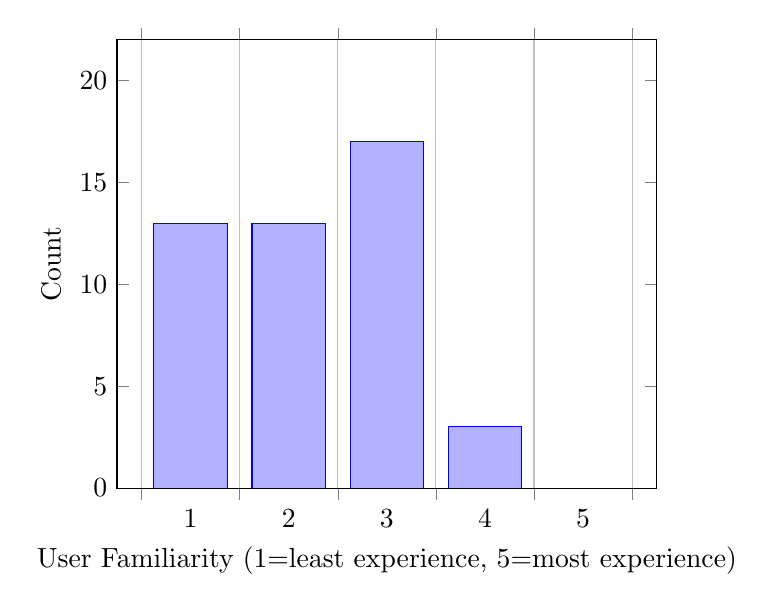
\begin{tikzpicture}
        \begin{axis}[ybar interval=0.75, xlabel={User Familiarity (1=least experience, 5=most experience)}, align=center, enlargelimits=0.05, ylabel=Count, area style, ymin=0, ymax=20, enlarge y limits={upper=0}]
            \addplot+[ybar interval, mark=no] plot coordinates { (1, 13) (2, 13) (3, 17) (4, 3) (5, 0) (6, 0) };
        \end{axis}
    \end{tikzpicture}
    \caption{User familiarity with gear design knowledge (A20).}
    \label{fig:gear_design}
\end{figure}

In terms of experience with gear design in CAD software, such as SolidWorks, the ratings were higher, with 74\% of users rating themselves slightly experienced or moderately experienced (two or three rating), with a mean rating of 2.43 (Figure~\ref{fig:gear_sw}). Since this study was conducted with the class nearing completion, these ratings were expected to be higher than if we ran the study at the beginning of the class since this is the first class in which they would learn how to use SolidWorks.

\begin{figure}
    \centering
    
    %\includegraphics[width=1\textwidth]{gear_sw}
    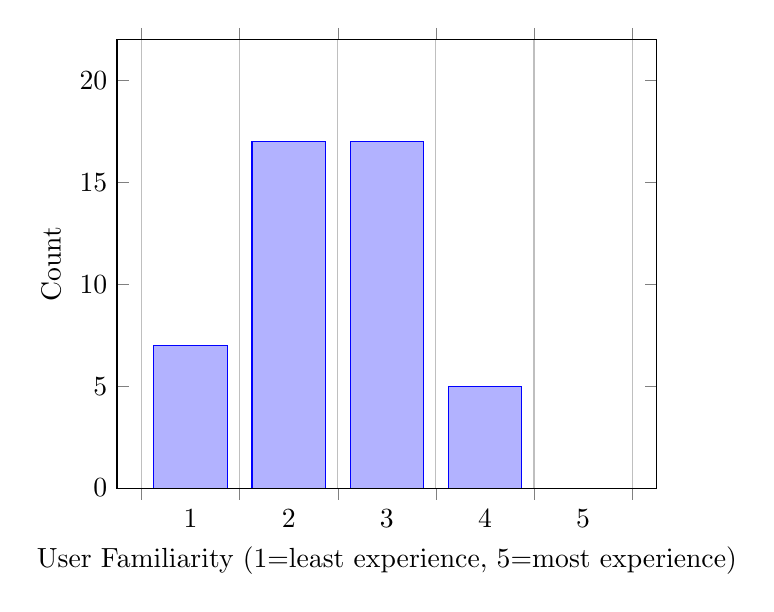
\begin{tikzpicture}
        \begin{axis}[ybar interval=0.75, xlabel={User Familiarity (1=least experience, 5=most experience)}, align=center, enlargelimits=0.05, ylabel=Count, area style, ymin=0, ymax=20, enlarge y limits={upper=0}]
            \addplot+[ybar interval, mark=no] plot coordinates { (1, 7) (2, 17) (3, 17) (4, 5) (5, 0) (6, 0) };
        \end{axis}
    \end{tikzpicture}
    \caption{User familiarity with gear design software (such as SolidWorks) (A20).}
    \label{fig:gear_sw}
\end{figure}

\subsubsection{User Feedback}

Once the participants completed the task, they were given another survey to complete. While the initial survey was focused on gathering basic information about the participants, this latter survey was focused on their experience using the software. The data from this survey gave us information about what we should change (or keep the same) in the new GearTrain system.

Before asking any feedback questions, we asked some basic information about the task itself, such as if they were able to complete it and how long it took. A histogram of the task duration can be found in Figure~\ref{fig:hist_time}. The average time to complete the task was 8 minutes and 58 seconds and the standard deviation was 3.93. The average difficulty rating of the task was 1.76, and the average difficulty rating for modifying the gear data was 1.7 (Figures~\ref{fig:a20_difficulty} and \ref{fig:a20_difficulty_mod}).

\begin{figure}[htbp]
    \centering
    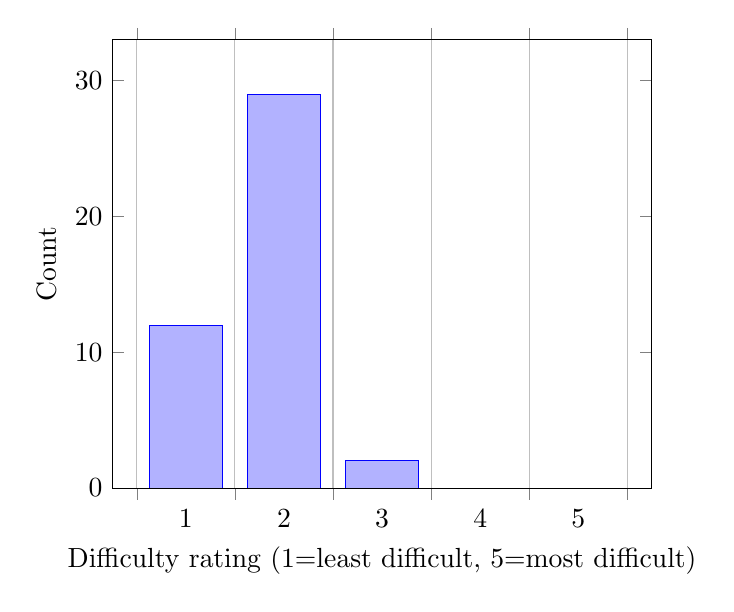
\begin{tikzpicture}
        \begin{axis}[ybar interval=0.75, xlabel={Difficulty rating (1=least difficult, 5=most difficult)}, align=center, enlargelimits=0.05, ylabel=Count, area style, ymin=0, ymax=30, enlarge y limits={upper=0}]
            \addplot+[ybar interval, mark=no] plot coordinates { (1, 12) (2, 29) (3, 2) (4, 0) (5, 0) (6, 0) };
        \end{axis}
    \end{tikzpicture}
    \caption{Task difficulty rating (A20).}
    \label{fig:a20_difficulty}
\end{figure}

\begin{figure}[htbp]
    \centering
    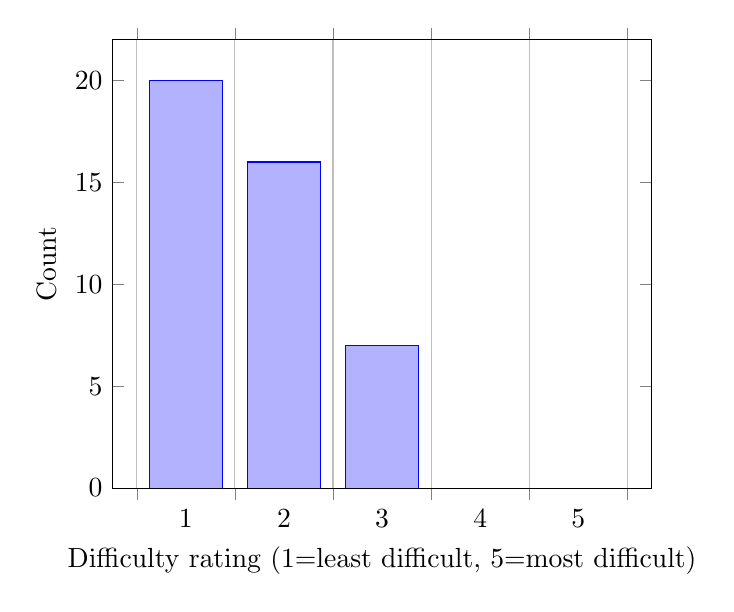
\begin{tikzpicture}
        \begin{axis}[ybar interval=0.75, xlabel={Difficulty rating (1=least difficult, 5=most difficult)}, align=center, enlargelimits=0.05, ylabel=Count, area style, ymin=0, ymax=20, enlarge y limits={upper=0}]
            \addplot+[ybar interval, mark=no] plot coordinates { (1, 20) (2, 16) (3, 7) (4, 0) (5, 0) (6, 0) };
        \end{axis}
    \end{tikzpicture}
    \caption{Gear modification difficulty rating (A20).}
    \label{fig:a20_difficulty_mod}
\end{figure}

\begin{figure}[htbp]
    \centering
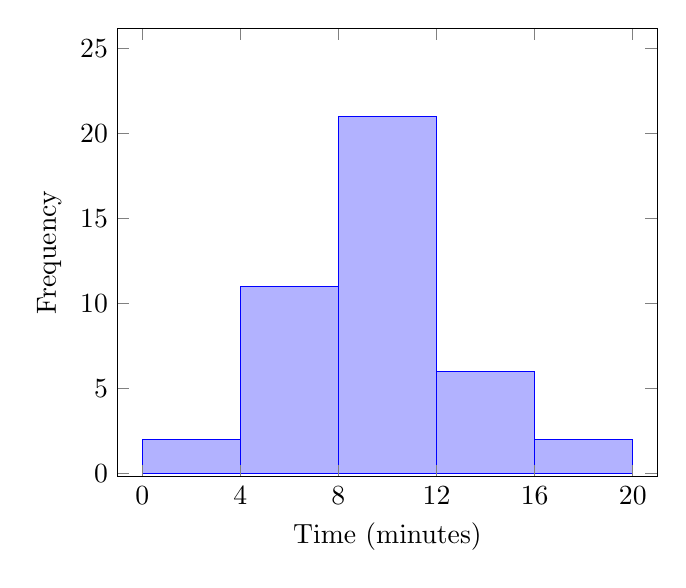
\begin{tikzpicture}
    \begin{axis}[xlabel=Time (minutes), ylabel=Frequency, area style, enlargelimits=0.05, ymax=25, xtick={0,4,8,12,16,20}]
        \addplot+[ybar interval, mark=no] plot coordinates { (0, 2) (4, 11) (8, 21) (12, 6) (16, 2) (20, 1) };
    \end{axis}
\end{tikzpicture}
    \caption{Histogram of time taken to complete the gear design task (A20).}
    \label{fig:hist_time}
\end{figure}

Since most of the responses are open response, where users could type anything they wanted, they needed to be categorized first before they were analyzed. There were a few categories of responses for each question, which will be detailed below. Note that the number of responses for each question does not match the total number of study participants since no open response questions were required, so some participants did not answer them. 37 participants (86\%) answered the question asking about what they found easy, while only 22 participants (51\%) answered the question asking what they found difficult. Finally, 37 participants (86\%) answered the question asking for recommended changes in the system.

\begin{singlespace}
\textbf{What about the gear design software did you find easy, if anything?}
\begin{itemize}
    \item Ease of use: 18/37 (48.6\%) of users said that tasks in the software were easy, including inputting gear data and generating in SolidWorks.
    \item User interface: 11/37 (29.7\%) of users liked the interface and thought it was easy to understand and found everything they needed to complete the task.
    \item Program functionality: 8/37 (21.6\%) of users thought the software in general was easy to use, especially when compared to designing gears by hand.
\end{itemize}

\textbf{What about the gear design software did you find difficult, if anything?}
\begin{itemize}
    \item Tutorial: 8/22 (36.4\%) of users found the tutorial difficult or did not know enough about gears to know what they were doing. This is a problem with the tutorial, and not the program, however.
    \item Program issues: 12/22 (54.5\%) of users had issues in the program that preventing them from completing the task properly. Some users also said that there was too much information to enter or that the program was not very user friendly.
    \item Installation: 2/22 (9.1\%) of users had problems installing or downloading the software, mainly due to antivirus problems.
\end{itemize}

\textbf{What would you change in the current system to make it easier to use or more functional?}
\begin{itemize}
    \item Explanation of terms: 4/34 (11.8\%) of users would have liked some basic help functions, like tooltips on hover or explanation of what certain gear terms mean, such as pitch angle.
    \item User interface: 9/34 (26.5\%) of users would prefer updates to the user interface, including making the application more visual and less text-based.
    \item User experience: 17/34 (50\%) of users wanted improvements to the user experience, many of which said they would like some sort of preview of the gear train before it is generated in SolidWorks.
    \item Tutorial: 3/34 (8.8\%) of users recommended some clarifications in the tutorial document to make the task easier to complete.
\end{itemize}

\end{singlespace}

Many users responded that there were problems with the tutorial document, which could have affected the study results. The document had a lot of steps for the user to complete and a lot of data to input (see Appendix~\ref{app:tutorial}), but the users were able to ask questions at any time. There was also a live demo of the program where the tutorial was walked through. Many of the comments about the tutorial are not about the tutorial itself being confusing, but rather they are about not knowing where this data comes from in the first place or what it means. Because of this, we believe that the quality of the tutorial document itself did not negatively affect the study results.

\subsection{GearTrain Study}

Two separate studies were run using the system made for this project, named ``GearTrain''. The first was run in the Modeling and Analysis of Mechatronic Systems (ME 4322) class at Worcester Polytechnic Institute during the last week of C term (March 2021). The second was run in the Advanced Engineering Design (ME 4320) and the Introduction to Engineering Design (ME 2300) classes during the third week of D term (April 2021). These studies will be referred to in this section as the C21 and D21 studies, respectively. Since these studies have different population demographics, their data will be analyzed separately to see if the results are different based on the participant's past experience.

\subsubsection{C21 Study}

This study was conducted in a Mechatronic Systems class as described above. A total of 25 students participated in the study. As in the A20 study, the participants were given a short task to complete using the software. In order to better gauge the learnability and ease of use of the system, the whole tutorial was modified from the A20 one. In this tutorial, the participant is given less guidance when completing the task to see if they can complete it without a lot of help. This was to test the learnability of the software, since we want the software to be intuitively easy to use. Additionally, a second task was added to be completed after the first. This task offered \emph{no guidance whatsoever}, and the participant was required to use what they learned so far to complete the task on their own, using the help website if needed. The full tutorial document for this study can be found in Appendix~\ref{app:tutorial}.

\paragraph{User Demographics for C21 Study}
In contrast with the A20 study, most of the participants in this study were juniors and seniors, with no freshman (Figure~\ref{fig:grades_first}). This is understandable since this is a more advanced Mechanical Engineering (ME) course so freshman do not have the prerequisite courses completed yet. Additionally, since this is a more advanced course, most of the students are mechanical engineering students (Figure~\ref{fig:majors_first}). Note that many of the students are double-majors. Unlike the Introduction to CAD class used in the A20 study, non-ME majors would have no reason to take this course because it does not relate to their major study. An Introduction to CAD class could be taken by other majors since they may need to use CAD in their field of study.

\begin{figure}[htbp]
    \centering
    \begin{tikzpicture}
        \pie{4.2/Sophomore,58.3/Junior,37.5/Senior}
    \end{tikzpicture}
    \caption{Year breakdown of study participants (C21, total=24).}
    \label{fig:grades_first}
\end{figure}

\begin{figure}[htbp]
    \centering
    \begin{tikzpicture}
        \pie{70.8/Mechanical Engineering (ME),12.5/Robotics Engineering (RBE),8.3/ME+RBE,8.4/ME+Other}
    \end{tikzpicture}
    \caption{Study participant majors (C21, total=24).}
    \label{fig:majors_first}
\end{figure}

\paragraph{Previous Experience}
Since Mechatronic Systems is a more advanced ME course, we expected many more participants to be familiar with gear design than the previous study (A20) since gears are used often by mechanical engineers. Similar to the previous system (A20), knowledge of gears is not required to use this program, but it may help the users understand the data they are entering for the tutorial. Several participants in the previous study mentioned that they did not understand the data they were entering. As seen in Figure~\ref{fig:gear_first}, participants were generally more knowledgeable about gears than in the previous study (previous study is Figure~\ref{fig:gear_design}).

\begin{figure}[htbp]
    \centering
    %\includegraphics[width=1\textwidth]{gear_design}
    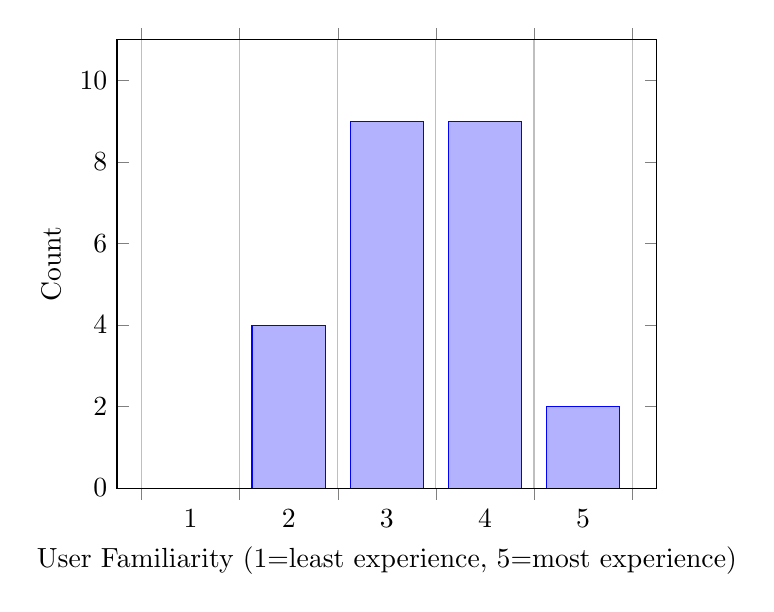
\begin{tikzpicture}
        \begin{axis}[ybar interval=0.75, xlabel={User Familiarity (1=least experience, 5=most experience)}, align=center, enlargelimits=0.05, ylabel=Count, area style, ymin=0, ymax=10, enlarge y limits={upper=0}]
            \addplot+[ybar interval, mark=no] plot coordinates { (1, 0) (2, 4) (3, 9) (4, 9) (5, 2) (6, 0) };
        \end{axis}
    \end{tikzpicture}
    \caption{User familiarity with gear design knowledge (C21).}
    \label{fig:gear_first}
\end{figure}

The mean familiarity rating was 3.375 (standard deviation 0.875), much higher than the average of 2.22 in the previous study. This was expected to be higher since the study was run in an advanced ME course with students who most likely have used gears at some point in their studies. Additionally, since the study was run at the end of the course rather than the beginning, the results are expected to be higher since the students can use what they learned from the course to aid them in the task.

Similarly, we expected that users are more experienced with CAD (Figure~\ref{fig:cad_first}). Even though knowledge of CAD is not required for this program, users who have used CAD may be more familiar with manipulating the 3D viewer of our software since it has similar controls to SolidWorks. The mean familiarity with CAD was 3.95 (standard deviation 0.806), much higher than the previous study value of 2.43. Again, this is expected since this is an advanced ME course. The previous study was run in an introduction to CAD course, where students are expected to have little to no experience using CAD.

\begin{figure}
    \centering
    %\includegraphics[width=1\textwidth]{gear_design}
    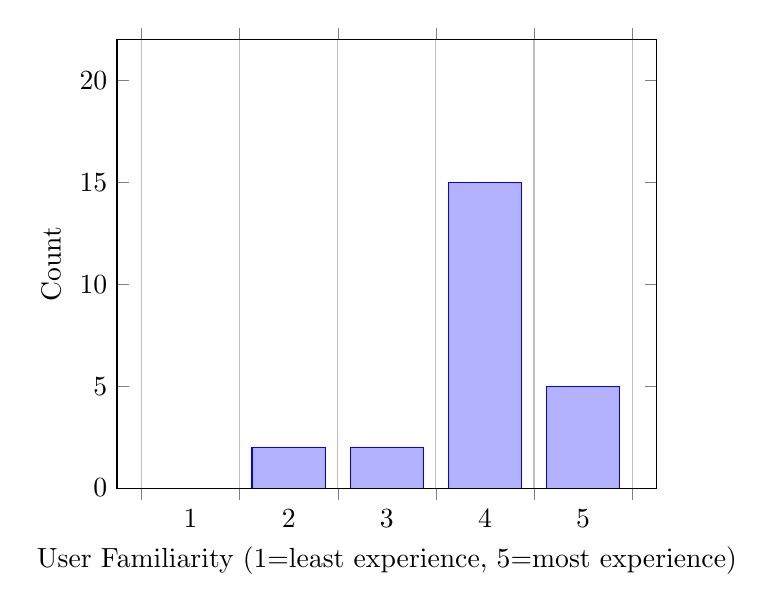
\begin{tikzpicture}
        \begin{axis}[ybar interval=0.75, xlabel={User Familiarity (1=least experience, 5=most experience)}, align=center, enlargelimits=0.05, ylabel=Count, area style, ymin=0, ymax=20, enlarge y limits={upper=0}]
            \addplot+[ybar interval, mark=no] plot coordinates { (1, 0) (2, 2) (3, 2) (4, 15) (5, 5) (6, 0) };
        \end{axis}
    \end{tikzpicture}
    \caption{User familiarity with CAD (e.g., SolidWorks, AutoCAD) (C21).}
    \label{fig:cad_first}
\end{figure}

\paragraph{User Feedback}
Similar to the previous study (A20), after the task was complete, the participants were required to complete another survey. This survey asked questions about their use of the software, such as what they found easy, what they found hard, and any features they wanted added. Before those questions, we asked approximately how long it took to complete the task. This is important for our program because we do not want users spending too much time doing simple tasks, as the whole point of the software is to save time designing gear trains. Overall, this task took longer than in the previous study. However, this task was also much longer since they needed to create two gear train designs instead of one. Figure~\ref{fig:time_hist1} shows a histogram of time taken to complete the task. Unlike the previous study, nobody was able to finish the task in less than five minutes. Some people also took more than 20 minutes to finish (some also took more than 30 minutes), unlike in the last study where the greatest amount of time was 20 minutes. The rightmost two bars in Figure~\ref{fig:time_hist1} are wider than the rest of the bars in the graph. This is because the users were asked for a range of time (0-5 minutes, 10-15 minutes, etc.), but one of the ranges was 20-30 minutes (10 minute range instead of 5 minutes), so the bar will be wider. One of them was also ``More than 30 minutes'', so this one is also wider.

\begin{figure}[htbp]
    \centering
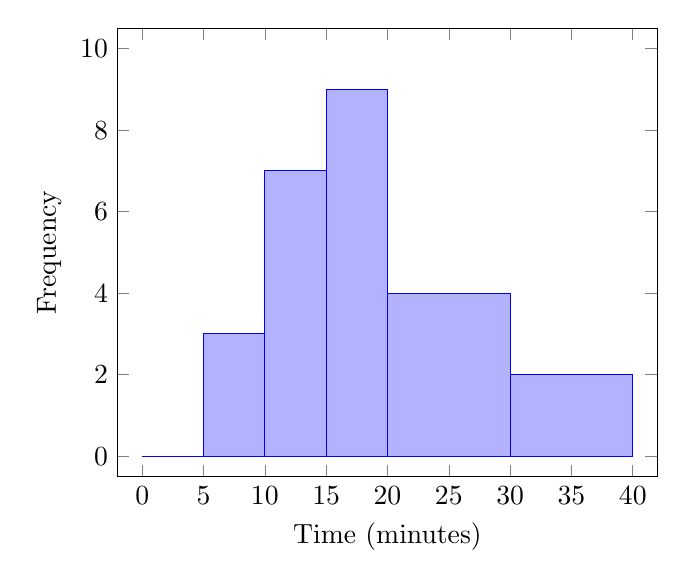
\begin{tikzpicture}
    \begin{axis}[xlabel=Time (minutes), ylabel=Frequency, area style, enlargelimits=0.05, ymax=10, xtick={0,5,10,15,20,25,30,35,40}]
        \addplot+[ybar interval, mark=no] plot coordinates { (0, 0) (5, 3) (10, 7) (15, 9) (20, 4) (30, 2) (40, 0)};
    \end{axis}
\end{tikzpicture}
    \caption{Histogram of time taken to complete the gear design task (C21).}
    \label{fig:time_hist1}
\end{figure}

Most users found the tutorial easy to complete (Figure~\ref{fig:difficulty1}). All users except one said that they were able to complete the tutorial (one participant was having difficulties with the remote desktop that prevented SolidWorks from opening). Compared to the old system, our program seems to be easier to use. Most users reported that modifying the gear data was easy, while rating program navigation a little more difficult. The average gear modification difficulty rating is 1.44 (standard deviation 0.51), while the average navigation difficulty rating is 1.8 (standard deviation 0.65). The old system's (A20 study) average gear modification difficulty rating was 1.7, making it slightly more difficult than GearTrain.

\begin{figure}[htbp]
    \centering
    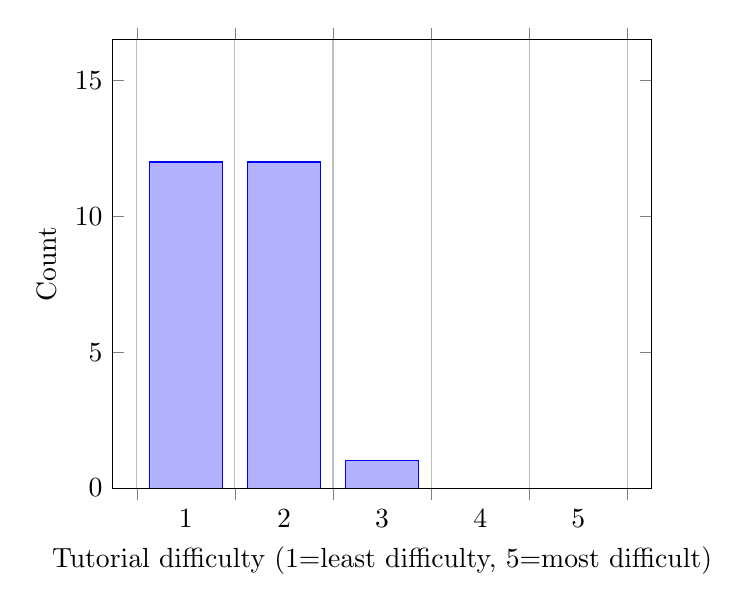
\begin{tikzpicture}
        \begin{axis}[ybar interval=0.75, xlabel={Tutorial difficulty (1=least difficulty, 5=most difficult)}, align=center, enlargelimits=0.05, ylabel=Count, area style, ymin=0, ymax=15, enlarge y limits={upper=0}]
            \addplot+[ybar interval, mark=no] plot coordinates { (1, 12) (2, 12) (3, 1) (4, 0) (5, 0) (6, 0) };
        \end{axis}
    \end{tikzpicture}
    \caption{Tutorial difficulty rating (C21).}
    \label{fig:difficulty1}
\end{figure}

Most users reported that they were satisfied with the look and feel of the program (average satisfaction rating 3.8/5, standard deviation 1.08). Our development time was mainly focused on user interface design, so we would expect that users would be satisfied with the interface. A question was added to the survey asking whether the 3D viewer improved their experience with the software. Since many of the participants of the old study requested a 3D viewer, it was important to know whether this was actually helpful. One hundred percent of users reported that the 3D viewer improved their experience with the program.

A help website was also created for this system in case the users needed help with any features or want to see what the program is capable of. No users reported needing to consult the help website, and everyone was able to successfully complete the tutorial (except for one due to a technical problem on the computer they were using). This strongly indicates the learnability and ease of use of our program since all participants were able to complete each task without help.

Study participants were also asked \emph{free response} questions, where they were able to give their feedback. These answers cannot be analyzed simply. Similar to how it was done before, the written responses for each question were categorized so they can be analyzed based on common factors, such as ease of use. The analysis of these answers is below, while full question answers can be found in Appendix~\ref{app:survey}.

Similar to the A20 study, responses to the free response questions were not required. In general, a higher percentage of participants responded to these questions compared to the A20 study. Twenty-four participants (96\%) of participants answered the question asking what they found easy, and 25 participants (100\%) of participants answered the question asking what they found difficult. Only 14 (56\%) of the responding participants recommended changes to the software.

\begin{singlespace}
\textbf{What about the software did you find easy?}
\begin{itemize}
    \item Ease of use: 11/24 (45.8\%) of users said that tasks in the software were easy, including inputting gear data and generating in SolidWorks.
    \item User interface: 7/24 (29.2\%) of users liked the interface and found it easy to use.
    \item Program features: 6/24 (25\%) of users liked the program features and found them easy to use, especially in regards to auto meshing.
\end{itemize}

\textbf{What about the software did you find difficult?}
\begin{itemize}
    \item Nothing: 6/25 (24\%) of users found nothing difficult with the program.
    \item Ease of use: 7/25 (28\%) of users had trouble using the software, including issues with SolidWorks generation (known bug at the time of the study) and other miscellaneous issues.
    \item User interface: 7/25 (28\%) of users found the interface difficult to use or were confused by certain parts of it.
    \item Program features: 5/25 (20\%) of users had miscellaneous issues with the software, including the aforementioned SolidWorks issue
\end{itemize}

\textbf{If you could change/add/remove anything in the software, what would it be?}
\begin{itemize}
    \item Interface changes: 7/14 (50\%) of users recommended changes to the interface to make it easier to use or less confusing (discussed in Chapter~\ref{sec:eval})
    \item SolidWorks: 2/14 (14.3\%) of users recommended bug fixes and changes to the SolidWorks generation part of the program
    \item Program features: 5/14 (35.7\%) of users recommended features to the program to improve its use for gear designers and to make it easier to use in general
\end{itemize}

\end{singlespace}

\subsubsection{D21 Study}
This study was conducted in an Introduction and an Advanced Engineering Design class as described previously. A total of 62 students participated in the study. Similar to the C21 study, the participants were given two short tasks to complete using the software. The first one was guided by giving the user exact instructions, while the second one was unguided since the user was not given any help regarding completing the task. The full tutorial document for this study can be found in Appendix~\ref{app:tutorial}.

\paragraph{User Demographics for D21 Study}

The demographics for this study were similar to the C21 study, with no freshmen participating (Figure~\ref{fig:grades_second}). In contrast to the C21 study, there was a more diverse group of upperclassmen major fields (Figure~\ref{fig:majors_second}). This could be because one of the classes in this study, Introduction to Engineering Design, is a less advanced class, so it may have more non-Mechanical Engineering students taking it.

\begin{figure}[htbp]
    \centering
    \begin{tikzpicture}
        \pie{35.6/Sophomore,37.8/Junior,26.6/Senior}
    \end{tikzpicture}
    \caption{Year breakdown of study participants (D21, total=62).}
    \label{fig:grades_second}
\end{figure}

\begin{figure}[htbp]
    \centering
    \begin{tikzpicture}
        \pie{90/Mechanical Engineering (ME),8/Robotics Engineering (RBE),2/Other}
    \end{tikzpicture}
    \caption{Study participant majors (D21, total=74).}
    \label{fig:majors_second}
\end{figure}

\paragraph{Previous Experience}
Since the two courses overall had fewer seniors than the C21 study, we expected a smaller percentage of participants to be familiar with gear design since gear train design had not been taught yet in these courses. Similar to the previous studies (A20 and C21), knowledge of gears is not required to use the GearTrain program, but it may help the users understand the data they are entering for the tutorial. As seen in Figure~\ref{fig:gear_second}, participants were generally less knowledgeable about gears compared to the previous study in C21 (previous study is Figure~\ref{fig:gear_first}).

The mean familiarity rating was 2.45 (standard deviation 1.077), much lower than the average of 3.375 in the previous study (C21). This was expected to be lower since the study was run in two varying levels of classes with fewer seniors.

\begin{figure}[htbp]
    \centering
    %\includegraphics[width=1\textwidth]{gear_design}
    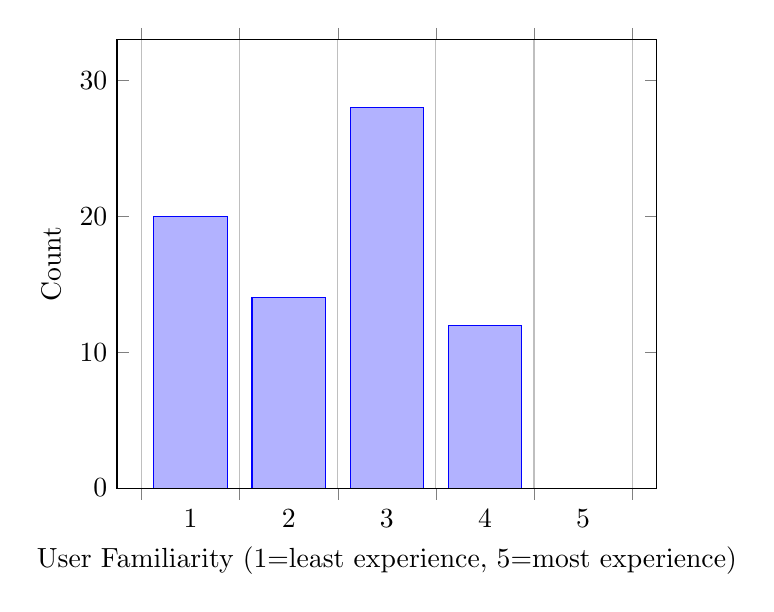
\begin{tikzpicture}
        \begin{axis}[ybar interval=0.75, xlabel={User Familiarity (1=least experience, 5=most experience)}, align=center, enlargelimits=0.05, ylabel=Count, area style, ymin=0, ymax=30, enlarge y limits={upper=0}]
            \addplot+[ybar interval, mark=no] plot coordinates { (1, 20) (2, 14) (3, 28) (4, 12) (5, 0) (6, 0) };
        \end{axis}
    \end{tikzpicture}
    \caption{User familiarity with gear design knowledge (D21).}
    \label{fig:gear_second}
\end{figure}

Similarly, we expected that users were less experienced with CAD (Figure~\ref{fig:cad_second}). While CAD knowledge  is not required for this program, having it would make users be more familiar with manipulating the 3D viewer of our application.  The mean familiarity with CAD was 3.42 (standard deviation 1.032), moderately lower than the previous study value of 3.95 Again, this is expected since there was an advanced and introductory course with varying degrees of knowledge and students. This meant there were more less-experienced students that could have brought the average down.

\begin{figure}
    \centering
    %\includegraphics[width=1\textwidth]{gear_design}
    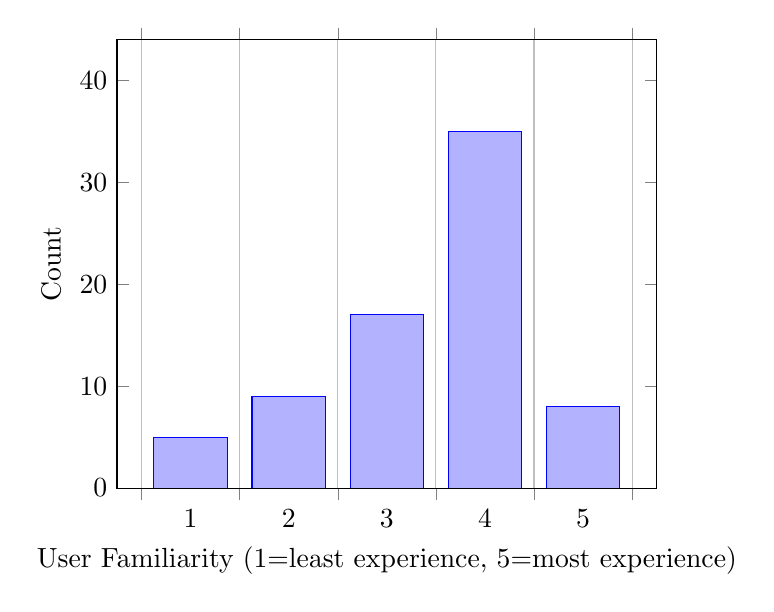
\begin{tikzpicture}
        \begin{axis}[ybar interval=0.75, xlabel={User Familiarity (1=least experience, 5=most experience)}, align=center, enlargelimits=0.05, ylabel=Count, area style, ymin=0, ymax=40, enlarge y limits={upper=0}]
            \addplot+[ybar interval, mark=no] plot coordinates { (1, 5) (2, 9) (3, 17) (4, 35) (5, 8) (6, 0) };
        \end{axis}
    \end{tikzpicture}
    \caption{User familiarity with CAD (e.g., SolidWorks, AutoCAD) (D21).}
    \label{fig:cad_second}
\end{figure}

\paragraph{User Feedback}

Similarly to the previous study (C21), after completing the tasks, the participants had to complete another survey. This survey asked questions about their use of the software, such as what they found easy, what they found hard, and any features they wanted added. Before those questions, we asked approximately how long it took to complete the task. Figure~\ref{fig:time_hist2} shows a histogram of time taken to complete the task. In contrast to the previous study, participants took much longer to complete the tasks. More than half of them took 20 minutes or longer. The average time to complete the tasks in the D21 study is higher than the C21 study because the users were less experienced than the C21 participants


\begin{figure}[htbp]
    \centering
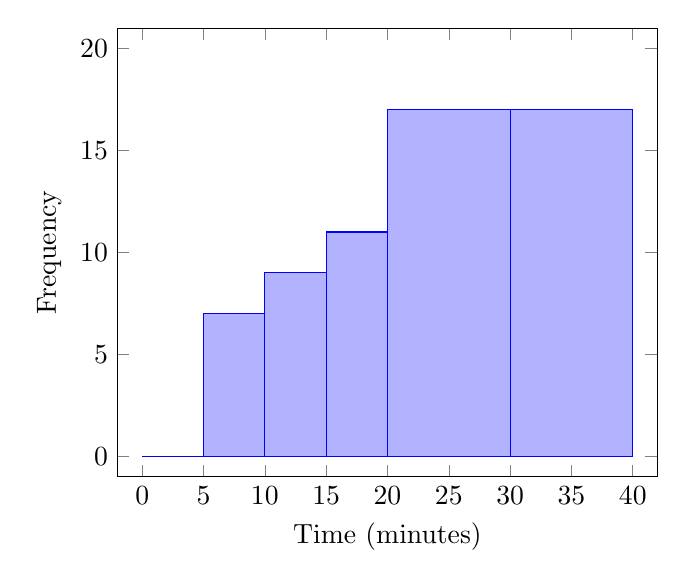
\begin{tikzpicture}
    \begin{axis}[xlabel=Time (minutes), ylabel=Frequency, area style, enlargelimits=0.05, ymax=20, xtick={0,5,10,15,20,25,30,35,40}]
        \addplot+[ybar interval, mark=no] plot coordinates { (0, 0) (5, 7) (10, 9) (15, 11) (20, 17) (30, 17) (40, 0)};
    \end{axis}
\end{tikzpicture}
    \caption{Histogram of time taken to complete the gear design task (D21).}
    \label{fig:time_hist2}
\end{figure}

Most users who completed the tutorial found it easy to complete (Figure~\ref{fig:difficulty2}). On the other hand, there were six participants who did not complete the study. This could have been due to issues with the remote server and bugs in the program that did not allow them to continue. Most users reported that modifying the gear data was easy, while rating program navigation a little more difficult. The average gear modification difficulty rating is 1.54 (standard deviation 0.84), while the average navigation difficulty rating is 1.85 (standard deviation 0.89). Most users reported that they were satisfied with the look and feel of the program (average satisfaction rating 3.96, standard deviation 1.05). We also asked how satisfied users were with the 3D viewer, since many participants from the A21 study requested it. 94\% percent found that the 3D viewer improved their experience with the software.

\begin{figure}[htbp]
    \centering
    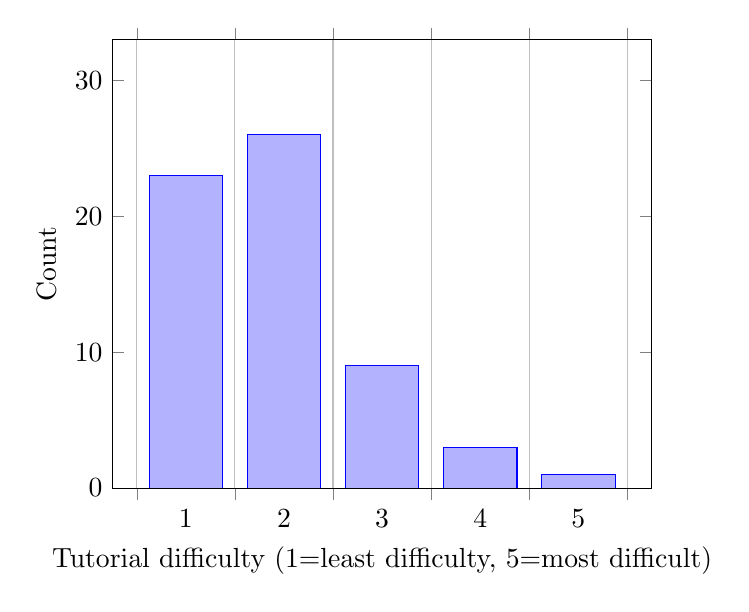
\begin{tikzpicture}
        \begin{axis}[ybar interval=0.75, xlabel={Tutorial difficulty (1=least difficulty, 5=most difficult)}, align=center, enlargelimits=0.05, ylabel=Count, area style, ymin=0, ymax=30, enlarge y limits={upper=0}]
            \addplot+[ybar interval, mark=no] plot coordinates { (1, 23) (2, 26) (3, 9) (4, 3) (5, 1) (6, 0) };
        \end{axis}
    \end{tikzpicture}
    \caption{Tutorial difficulty rating (D21).}
    \label{fig:difficulty2}
\end{figure}

A help website was also created for this system in case the users needed help with any features or want to see what the program is capable of. Unlike the previous study in C21, 21\% consulted the help website at least once. This makes sense, since their were more participants this time and the users had less experience.

Similar to the A20 and C21 study, responses to the free response questions were optional. In general, a lower percentage of participants responded to these questions compared to the C21 study. Fifty-eight participants (93\%) of participants answered the question asking what they found easy, and 26 participants (41\%) of participants answered the question asking what they found difficult. Only 11 (18\%) of participants recommended changes to the software. As with the other studies, all short answer responses can be found in Appendix~\ref{app:survey}.

\begin{singlespace}
\textbf{What about the software did you find easy?}
\begin{itemize}
    \item Ease of use: 24/59 (40.6\%) of users said that tasks in the software were easy, including inputting gear data and generating in SolidWorks.
    \item User interface: 18/59 (30.5\%) of users liked the interface and found it easy to use.
    \item Program features: 17/59 (28.8\%) of users liked the program features and found them easy to use, especially in regards to auto meshing.
\end{itemize}

\textbf{What about the software did you find difficult?}
\begin{itemize}
    \item Nothing: 9/26 (34.6\%) of users found nothing difficult with the program.
    \item Ease of use: 6/26 (23.1\%) of users had trouble using the software, including issues with SolidWorks generation (known bug at the time of the study) and other miscellaneous issues.
    \item User interface: 7/26 (26.9\%) of users found the interface difficult to use or were confused by when to save.
    \item Program features: 4/26 (15.3\%) of users had miscellaneous issues with the software, or importing a file.
\end{itemize}

\textbf{If you could change/add/remove anything in the software, what would it be?}
\begin{itemize}
    \item Interface changes: 5/11 (45.4\%) of users recommended changes to the interface to make it easier to use or less confusing (discussed in Chapter~\ref{sec:eval})
    \item SolidWorks: 3/11 (27.2\%) of users recommended bug fixes and changes to the SolidWorks generation part of the program
    \item Program features: 3/11 (27.2\%) of users recommended features to the program to improve its use for gear designers and have more features in general
\end{itemize}

\end{singlespace}


\end{doublespace}